
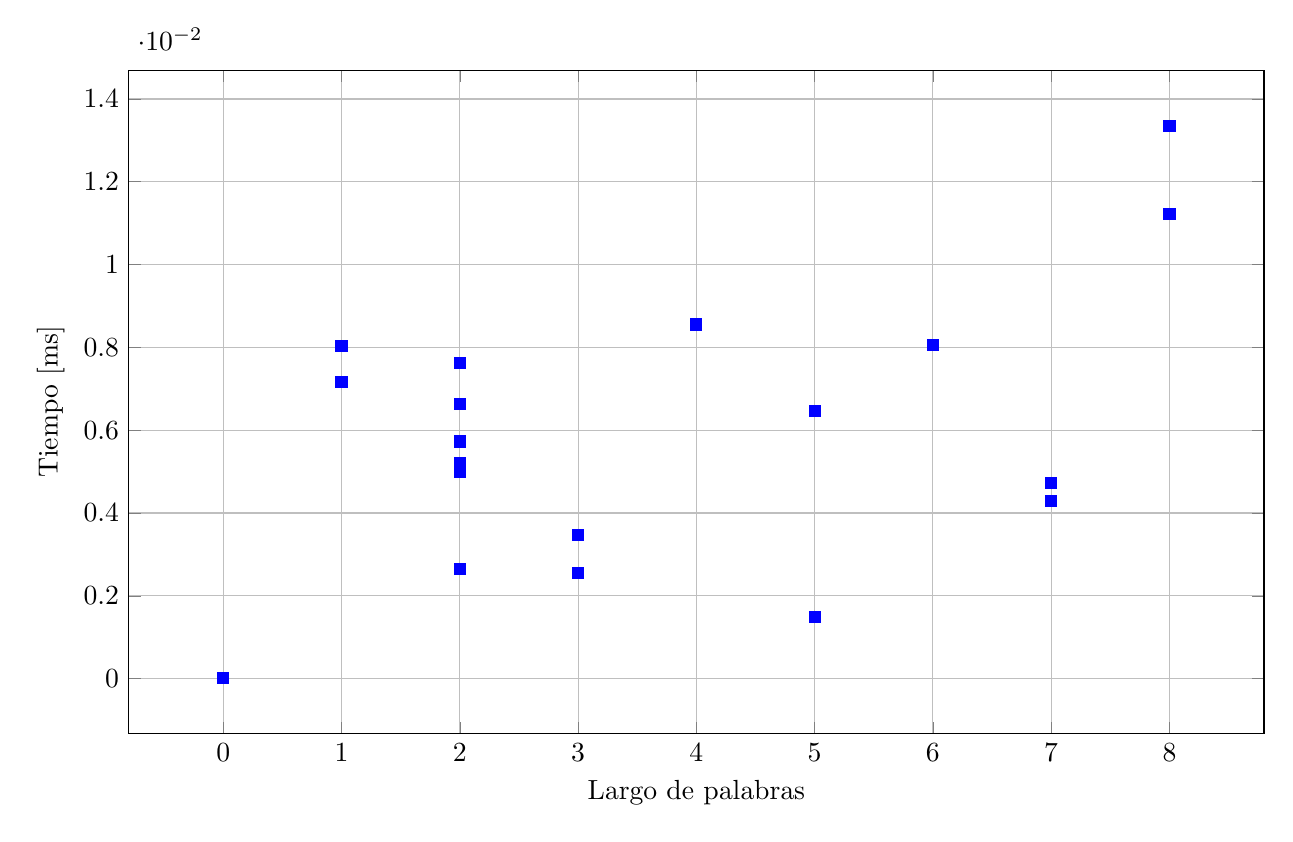
\begin{tikzpicture}
    %\begin{loglogaxis}[
    %\begin{semilogxaxis}[ % Cambiar a semilogxaxis    
    \begin{axis}[
        xlabel={Largo de palabras },
        ylabel={Tiempo [ms]},
        grid=major,
        legend pos=north west,
        legend cell align={left},
        width=16cm,
        height=10cm, 
        xtick=data,
    ]
    \addplot[blue, only marks, mark=square*] coordinates {
    (8, 0.011224)
    (5, 0.006471)
    (5, 0.001480)
    (3, 0.002552)
    (2, 0.002638)
    (3, 0.003478)
    (7, 0.004291)
    (7, 0.004733)
    (2, 0.005001)
    (2, 0.005213)
    (2, 0.005724)
    (2, 0.005742)
    (2, 0.006627)
    (1, 0.007173)
    (2, 0.007619)
    (6, 0.008050)
    (8, 0.013350)
    (4, 0.008553)
    (0, 0.000009)
    (1, 0.008032)
};
   
\end{axis}
%\end{semilogxaxis} % Cambiar a semilogxaxis
\end{tikzpicture}
